\documentclass[crop,class=article]{standalone}
%----------------------------Preamble-------------------------------%
\usepackage{amssymb}        % For \mathbb{C}.
\usepackage{tikz}           % Drawing/graphing tools.
\usetikzlibrary{
    arrows.meta,            % Latex and Stealth arrows.
    decorations.markings,   % Adding arrows in the middle of a line.
}
%--------------------------Main Document----------------------------%
\begin{document}
    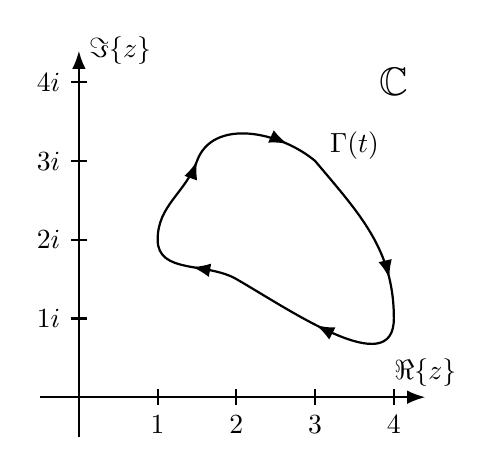
\begin{tikzpicture}[thick]
        % Axes:
        \draw[>=Latex, ->] (-0.5, 0) -- (4.4, 0) node[above] {$\Re\{z\}$};
        \draw[>=Latex, ->] (0, -0.5) -- (0, 4.4) node[right] {$\Im\{z\}$};
        % Axes labels:
        \foreach\n in {1,2,3,4}{%
            \draw (\n,3pt) -- (\n,-3pt) node [below] {$\n$};
            \draw (3pt,\n) -- (-3pt,\n) node [left] {$\n{i}$};
        }
        \begin{scope}[%
            >=Latex,
            ->-/.style={%
                decoration={%
                    markings,
                    mark=at position 0 with \arrow{>},
                    mark=at position .15 with \arrow{>},
                    mark=at position .4 with \arrow{>},
                    mark=at position .6 with \arrow{>},
                    mark=at position .8 with \arrow{>}
                },
                postaction={decorate}
            }
        ]
            \draw[->-]
                (1.5,3) to [out=70, in=140] (3,3)
                        to [out=-50, in=90] (4,1)
                        to [out=-90, in=-30] (2,1.5)
                        to [out=150, in=-90] (1,2)
                        to [out=90, in=-110] cycle;
        \end{scope}
        \node at (4,4) {\Large{$\mathbb{C}$}};
        \node at (3.5,3.2) {\normalsize{$\Gamma(t)$}};
    \end{tikzpicture}
\end{document}